%
% Complete documentation on the extended LaTeX markup used for Insight
% documentation is available in ``Documenting Insight'', which is part
% of the standard documentation for Insight.  It may be found online
% at:
%
%     http://www.itk.org/

\documentclass{InsightArticle}


%%%%%%%%%%%%%%%%%%%%%%%%%%%%%%%%%%%%%%%%%%%%%%%%%%%%%%%%%%%%%%%%%%
%
%  hyperref should be the last package to be loaded.
%
%%%%%%%%%%%%%%%%%%%%%%%%%%%%%%%%%%%%%%%%%%%%%%%%%%%%%%%%%%%%%%%%%%
\usepackage[dvips,
bookmarks,
bookmarksopen,
backref,
colorlinks,linkcolor={blue},citecolor={blue},urlcolor={blue},
]{hyperref}
% to be able to use options in graphics
\usepackage{graphicx}
% for pseudo code
\usepackage{listings}
% subfigures
\usepackage{subfigure}


%  This is a template for Papers to the Insight Journal. 
%  It is comparable to a technical report format.

% The title should be descriptive enough for people to be able to find
% the relevant document. 
\title{Tophap by area}

% 
% NOTE: This is the last number of the "handle" URL that 
% The Insight Journal assigns to your paper as part of the
% submission process. Please replace the number "1338" with
% the actual handle number that you get assigned.
%
\newcommand{\IJhandlerIDnumber}{3228}

% Increment the release number whenever significant changes are made.
% The author and/or editor can define 'significant' however they like.
% \release{0.00}

% At minimum, give your name and an email address.  You can include a
% snail-mail address if you like.
\author{Ga\"etan Lehmann{$^1$}}
\authoraddress{{$^1$}INRA, UMR 1198; ENVA; CNRS, FRE 2857, Biologie du
D\'eveloppement et 
Reproduction, Jouy en Josas, F-78350, France.}

\begin{document}


%
% Add hyperlink to the web location and license of the paper.
% The argument of this command is the handler identifier given
% by the Insight Journal to this paper.
% 
\IJhandlefooter{\IJhandlerIDnumber}

\maketitle

\ifhtml
\chapter*{Front Matter\label{front}}
\fi


\begin{abstract}
\noindent
The tophat transform is a well know and widely used transform based of morphological opening or closing.
It is often used to remove the background in an image, where the background is defined as the zones which do not fit in the user provided kernel.

Similarly, the tophat by area is used to remove the background in an image, but the criteria of selection is the size of the connected component,
either in physical size or in number of pixels, and is independant of the shape of the connected component. This property makes the tophat non
dependant of the shape of the object and makes easier to describe the criteria.
% Another important property of the tophat by area, inherited from the area opening used internally, is that it ensure to never add any edge in the image -- it only removes some of them.
\end{abstract}

\IJhandlenote{\IJhandlerIDnumber}

\tableofcontents

\section{Tophat by area}

The white tophat by area is used when the background is black to keep only the object smaller than the criteria provided by the user.
It is computed as
\begin{eqnarray}
whiteTophat = input - areaOpening(input)
\end{eqnarray}

The black tophat by area is used when the background is white. It is computed as
\begin{eqnarray}
blackTophat = input - areaClosing(input)
\end{eqnarray}

\begin{figure}[htbp]
\begin{center}
\subfigure[Input image.]{\includegraphics[scale=0.9]{cthead1}}
\subfigure[White area tophat.]{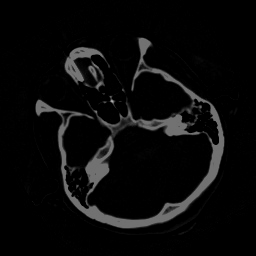
\includegraphics[scale=0.9]{white-1000-0-1}}
\subfigure[Black area tophat.]{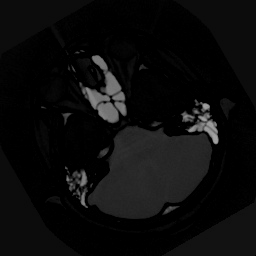
\includegraphics[scale=0.9]{black-1000-0-1}}
\caption{White and black tophat with a criteria of 1000, using image spacing and a 4-connectivity.}
\end{center}
\end{figure}

\section{Implementation}

The white tophat by area is implemented in \verb$itk::WhiteTopHatByAreaImageFilter$ and the black tophat by area in \verb$BlackTopHatByAreaImageFilter$.
They both provide the same options to the user:
\begin{itemize}
 \item \verb$Set/GetLambda()$ to set or retrietve the criteria;
 \item \verb$Set/GetUseImageSpacing()$ to set/get whether the image spacing should be used or not. If not used, the size of the connected components is
computed in pixels.
\end{itemize}

Here is an example of usage for the white tophat by area. The black tophap by area filter is used in the exact same way.

\small \begin{verbatim}
#include "itkImageFileReader.h"
#include "itkImageFileWriter.h"
#include "itkSimpleFilterWatcher.h"

#include "itkWhiteTopHatByAreaImageFilter.h"


int main(int argc, char * argv[])
{

  if( argc != 6 )
    {
    std::cerr << "usage: " << argv[0] << " intput output lambda connectivity useSpacing" << std::endl;
    std::cerr << " input: the input image" << std::endl;
    std::cerr << " output: the output image" << std::endl;
    // std::cerr << "  : " << std::endl;
    exit(1);
    }

  const int dim = 2;
  
  typedef unsigned char PType;
  typedef itk::Image< PType, dim > IType;

  typedef itk::ImageFileReader< IType > ReaderType;
  ReaderType::Pointer reader = ReaderType::New();
  reader->SetFileName( argv[1] );

  typedef itk::WhiteTopHatByAreaImageFilter< IType, IType > FilterType;
  FilterType::Pointer filter = FilterType::New();
  filter->SetInput( reader->GetOutput() );
  filter->SetLambda( atof(argv[3]) );
  filter->SetFullyConnected( atoi(argv[4]) );
  filter->SetUseImageSpacing( atoi(argv[5]) );

  itk::SimpleFilterWatcher watcher(filter, "filter");

  typedef itk::ImageFileWriter< IType > WriterType;
  WriterType::Pointer writer = WriterType::New();
  writer->SetInput( filter->GetOutput() );
  writer->SetFileName( argv[2] );
  writer->Update();

  return 0;
}
\end{verbatim} \normalsize

\section{Wrapping}

The two new filters are wrapped with WrapITK.
 
\appendix


\bibliographystyle{plain}
\bibliography{InsightJournal}
\nocite{ITKSoftwareGuide}
\nocite{Beare2007}

\end{document}

